\documentclass{beamer}
\usepackage[spanish]{babel}
\usepackage[utf8]{inputenc}
\usepackage{graphicx}
\usepackage{multimedia}
\usepackage{animate}
\usepackage{tcolorbox}
\usebackgroundtemplate{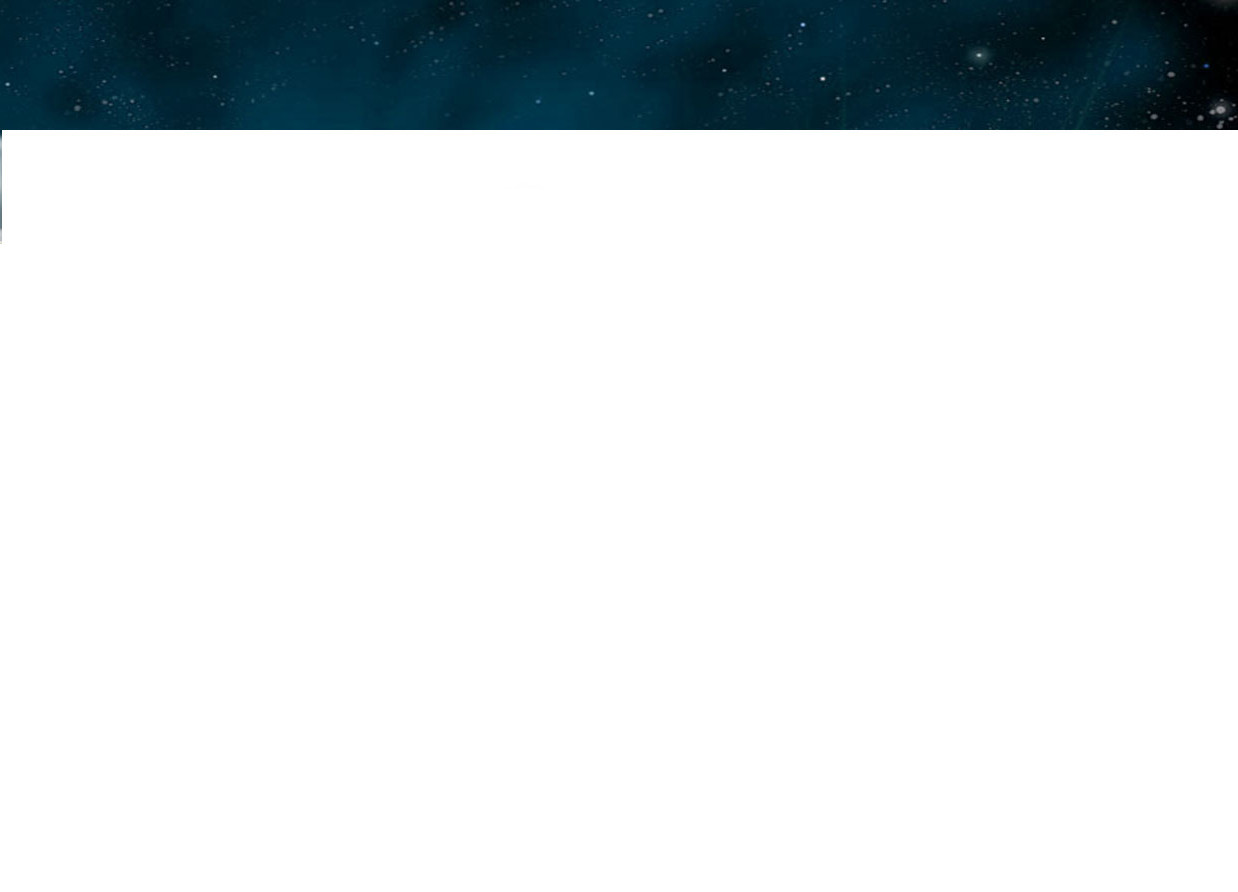
\includegraphics[width=\paperwidth]{sources/images/template_internal.jpg}}
\setbeamercolor{frametitle}{fg=white}
\usefonttheme{structuresmallcapsserif}
\setbeamertemplate{footline}[frame number]

\usepackage{default}

\newcounter{stepsBarnes}
\newcommand{\seti}{\setcounter{stepsBarnes}{\value{enumi}}}
\newcommand{\conti}{\setcounter{enumi}{\value{stepsBarnes}}}
\definecolor{green}{RGB}{0, 150, 0}

\begin{document}
{
	\usebackgroundtemplate{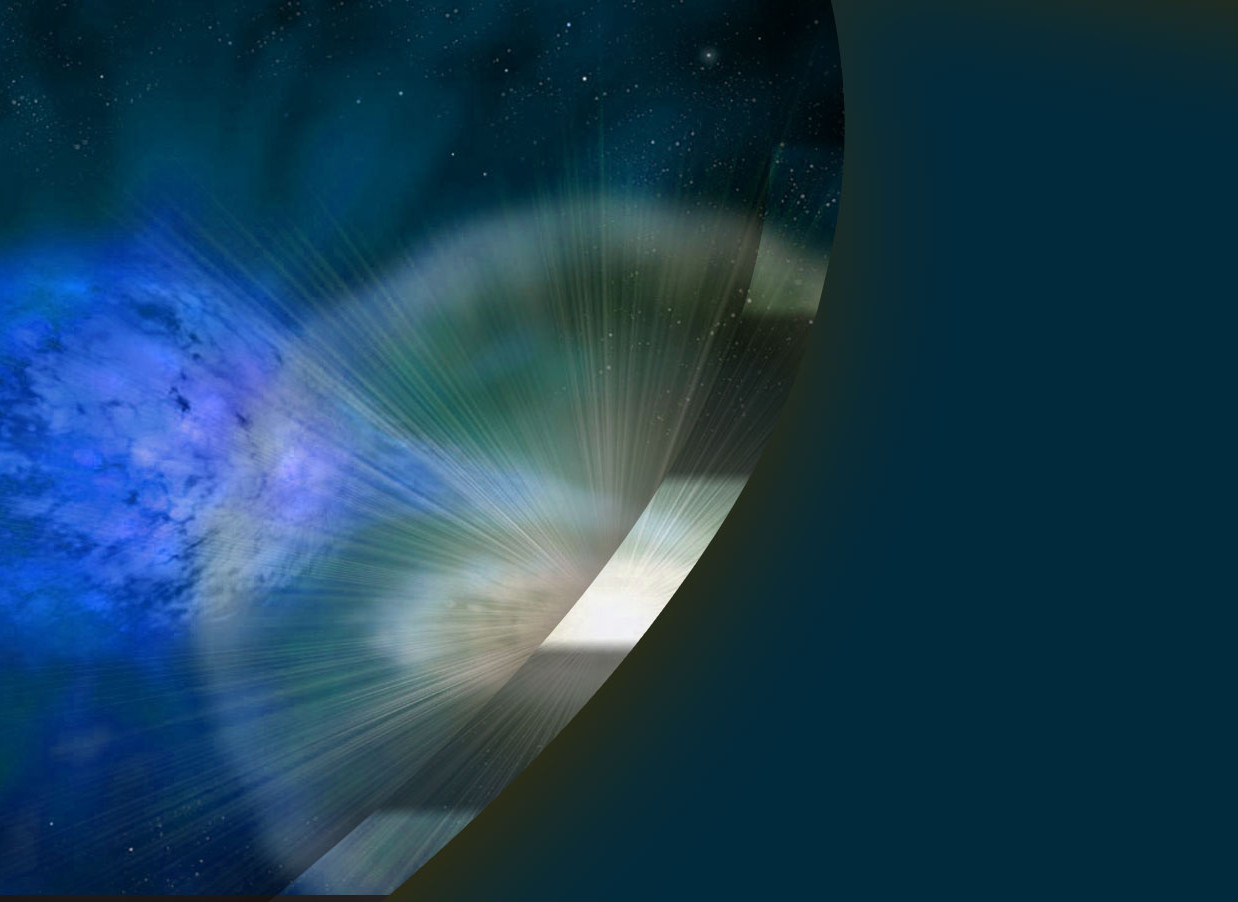
\includegraphics[width=\paperwidth]{sources/images/template_main.jpg}}
	\begin{frame}
		\centering
		\color{white}
		\textsc{\LARGE Dinámica de galaxias, una simulación con $N\log N$ iteraciones.}
		\\
		\vspace{5cm}
		\raggedleft Juan Barbosa
	\end{frame}
}

\begin{frame}{Introducci\'on}
	\centering
	\begin{columns}
		\begin{column}{.5\textwidth}
			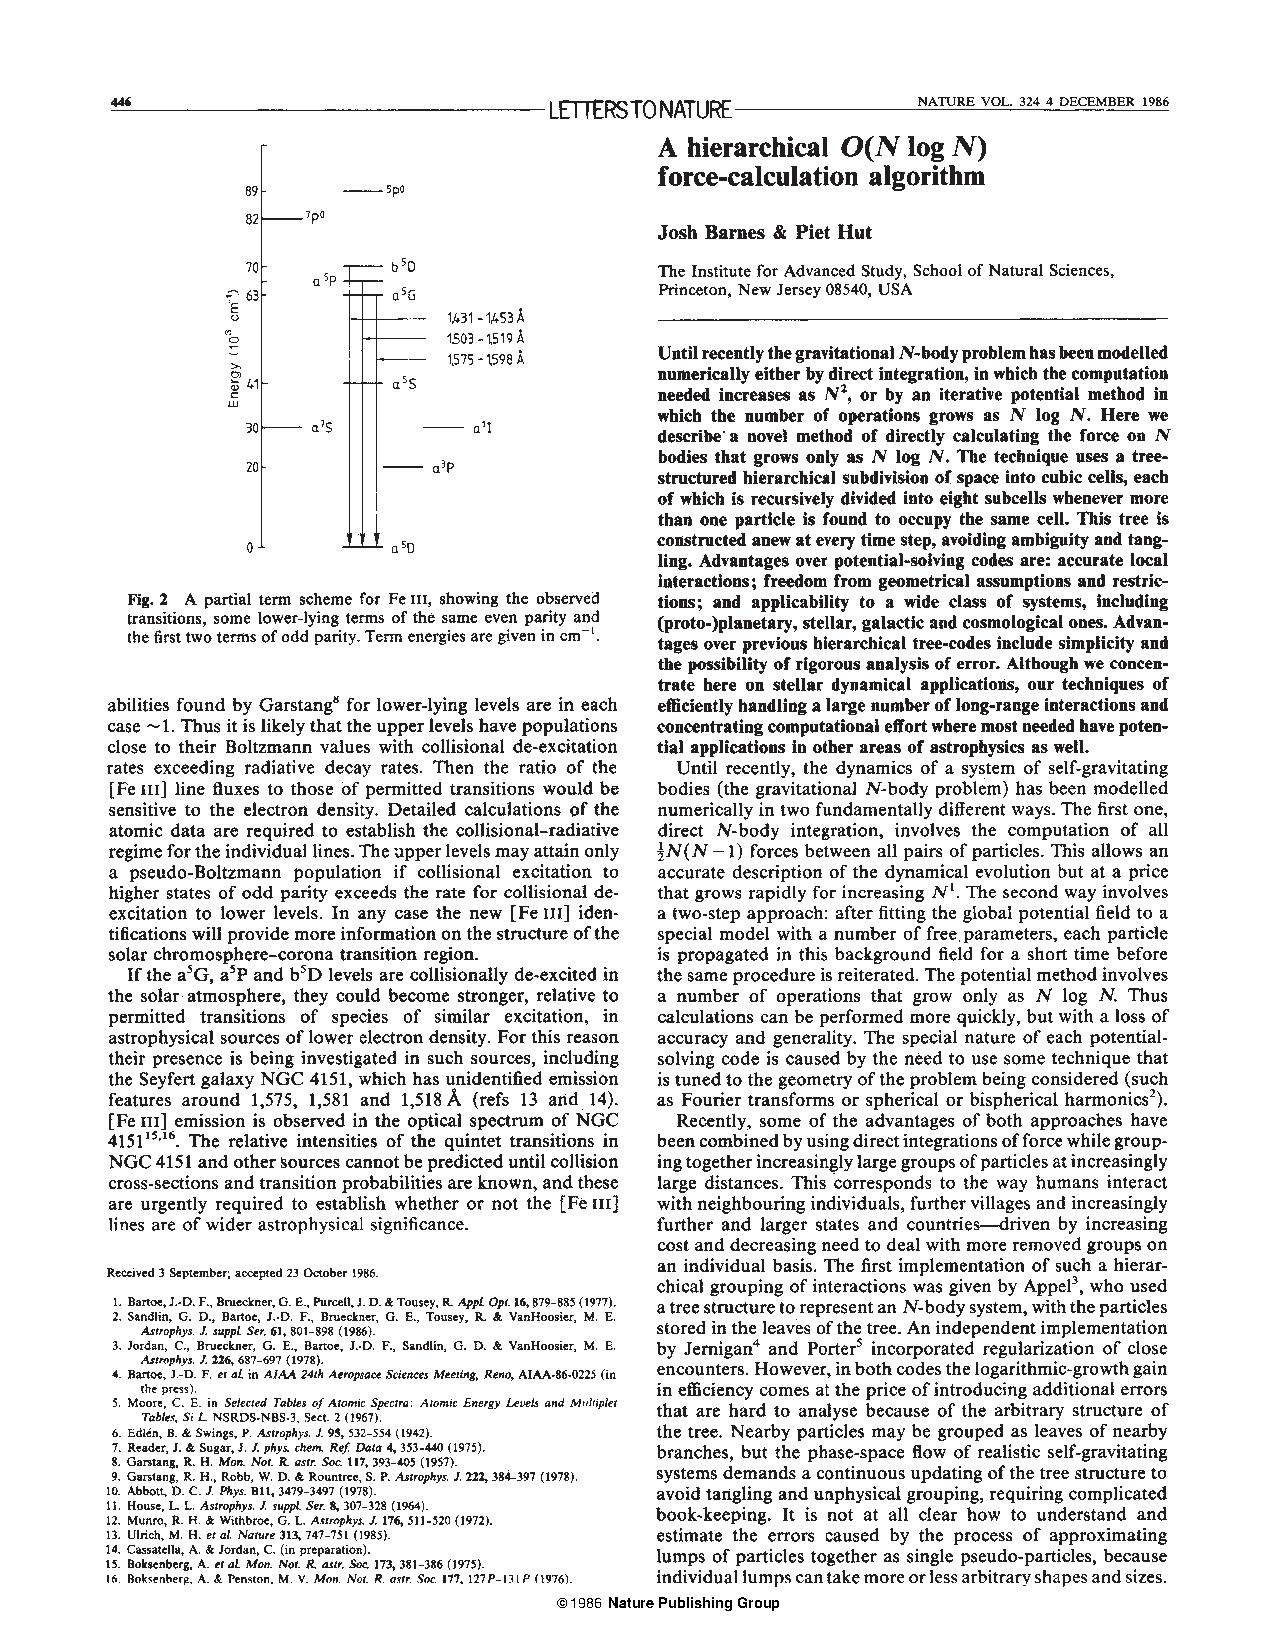
\includegraphics[height=0.8\textheight]{sources/images/barnes1986.pdf}
		\end{column}
		\begin{column}{.5\textwidth}
			\centering
			\begin{tabular}{cc}
				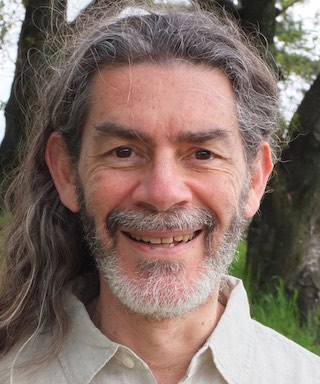
\includegraphics[height=0.3\textheight]{sources/images/barnes.jpg} & Josh Barnes\\
				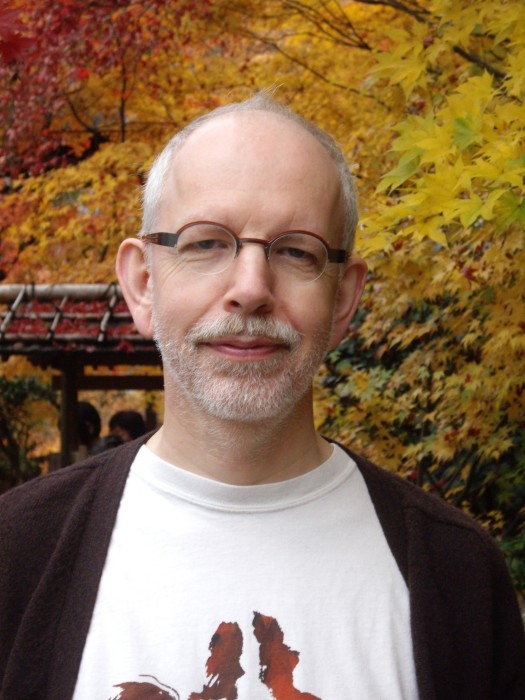
\includegraphics[height=0.3\textheight]{sources/images/hut.jpg}
				& Piet Hut \\
			\end{tabular}
		\end{column}
	\end{columns}
	
\end{frame}

\begin{frame}{Introducci\'on}
	\begin{columns}
		\begin{column}{.5\textwidth}
			\begin{tabular}{c}
				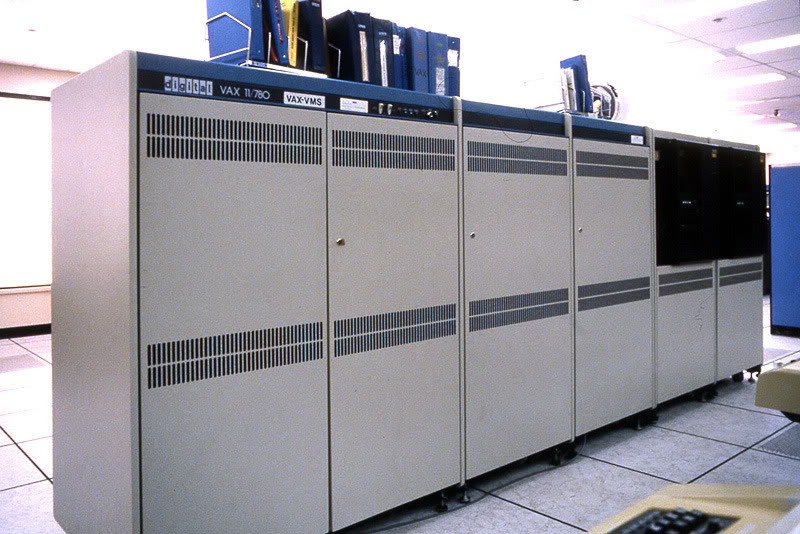
\includegraphics[width=\textwidth]{sources/images/DEC-VAX-11-780} \\
				VAX 11/780
			\end{tabular}
		\end{column}
		\begin{column}{.5\textwidth}
			\begin{itemize}
				\item<2-> Simulaci\'on con 4096 cuerpos.
				\item<3-> Tiempo: 10 horas de CPU.
			\end{itemize}
		\end{column}
	\end{columns}
\end{frame}
\begin{frame}{Funcionamiento}
	El algoritmo propuesto por Barnes y Hut consta de dos pasos fundamentales, la divisi\'on recursiva del espacio y la forma como se calcula la fuerza sobre un cuerpo. \pause
	\begin{enumerate}
		\item Divisi\'on jer\'arquica del espacio. \pause
		\seti
	\end{enumerate}
	\begin{columns}
		\begin{column}{0.5\linewidth}
			\centering
			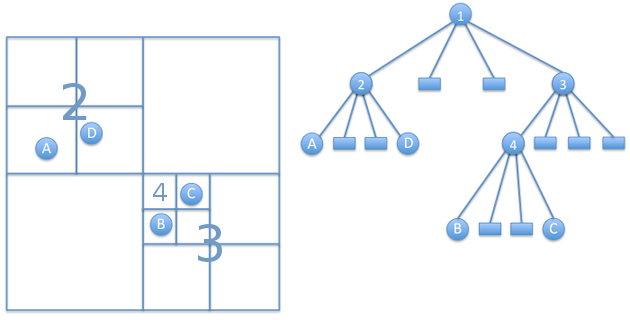
\includegraphics[width=\linewidth]{sources/images/quadtree.png}\\
			\'Arbol dos dimensional.\pause
		\end{column}
		\begin{column}{0.5\linewidth}
			\centering
			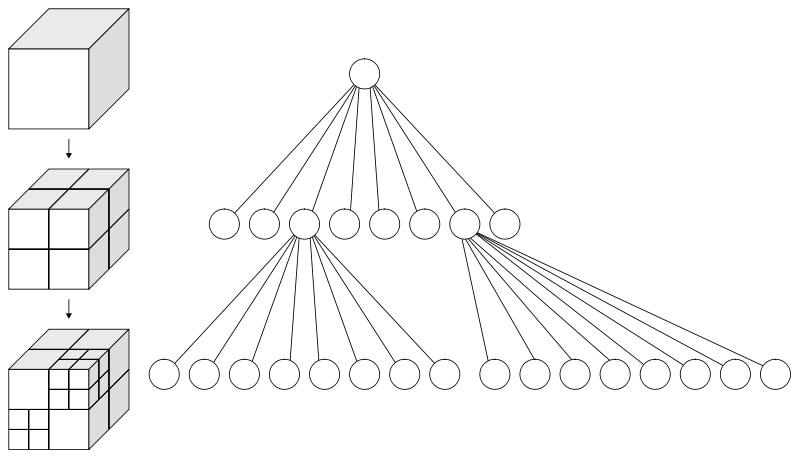
\includegraphics[width=\linewidth]{sources/images/octree.png}\\
			\'Arbol tridimensional.
		\end{column}
	\end{columns}
\end{frame}
\begin{frame}{Funcionamiento}
	\begin{enumerate}
		\conti
		\item Fuerza sobre un cuerpo.
	\end{enumerate}
	\small
	El n\'umero de iteraciones se reduce al considerar centros de masa y distancias. \pause
	\begin{itemize}
		\item Cada caja tiene una longitud espec\'ifica \pause
		\item Un centro de masa \pause
		\item Y la masa contenida \pause
	\end{itemize}
	\centering
	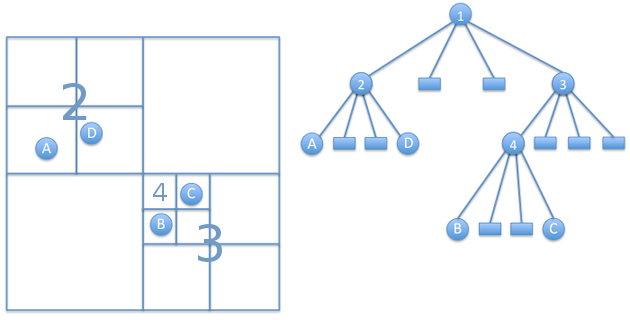
\includegraphics[width=0.5\linewidth]{sources/images/quadtree.png}
\end{frame}
\begin{frame}{Funcionamiento}
	\begin{columns}
		\begin{column}{0.6\textwidth}
			\centering
			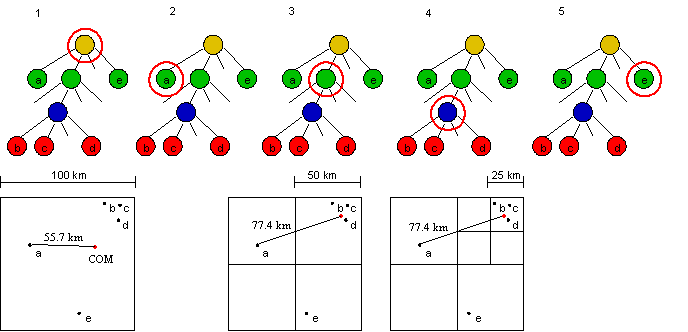
\includegraphics[width=\linewidth]{sources/images/force.png}\\
			\begin{itemize}
				\item Se define un coeficiente de precisi\'on.
			\end{itemize}
			$\tau = \dfrac{size}{distance} = 0.5$
			\pause
		\vspace{1cm}
		
		\end{column}
		\begin{column}{0.4\textwidth}
			\begin{enumerate}
				\footnotesize
				\item {\color{orange} Nodo principal} \pause
				\begin{equation*}
					\dfrac{s}{d} = \dfrac{100}{55.7} \approx 1.8 > \tau 
				\end{equation*}
				\pause
				\item {\color{green} Primer nodo} \pause
				\item {\color{green} Segundo nodo} \pause
				\begin{equation*}
					\dfrac{s}{d} = \dfrac{50}{77.4} \approx 0.6 > \tau
				\end{equation*}
				\pause
				\item {\color{blue} Segundo nodo} \pause
				\boxed{\dfrac{s}{d} = \dfrac{25}{77.4} \approx 0.3 < \tau}
				\pause
				\item {\color{green} Cuarto nodo} \pause
				\boxed{\text{Nodo externo, contribuye}}
			\end{enumerate}
		\end{column}
	\end{columns}
\end{frame}
\begin{frame}{Funcionamiento}
	La construcci\'on del arbol se realiza para cada instante de tiempo.
	\centering
	\movie[height = 0.55\textwidth, width = 0.8\textwidth, poster, showcontrols]{}{sources/animations/boxes_points.mp4}
	\\
	Observaci\'on
\end{frame}
\begin{frame}{Funcionamiento}
	La construcci\'on del arbol se realiza para cada instante de tiempo.
	\centering
	\movie[height = 0.55\textwidth, width = 0.8\textwidth,poster, showcontrols]{}{sources/animations/boxes.mp4}
	\\
	Todas las cajas
\end{frame}
\begin{frame}{Funcionamiento}
	La construcci\'on del arbol se realiza para cada instante de tiempo.
	\centering
	\movie[height = 0.55\textwidth, width = 0.8\textwidth, poster, showcontrols]{}{sources/animations/boxes_child_only.mp4}
	\\
	Cajas con una part\'icula
\end{frame}
\begin{frame}{Construcci\'on de una simulaci\'on}
	\begin{enumerate}
		\item Descripci\'on del sistema. \pause
		\item Condiciones iniciales. \pause
		\item Soluci\'on de las ecuaciones. \pause
		\item Visualizaci\'on.
	\end{enumerate}
\end{frame}
\begin{frame}{Descripci\'on del sistema}
	Usando la ley de gravitaci\'on universal:
	\begin{equation}
		\vec{F_i} = m_i\vec{a}_i = - \sum\limits_{j\neq i}^N G\dfrac{m_im_j}{|\vec{r}_{ij}|^3}\left(\vec{r}_i - \vec{r}_j\right)
	\end{equation}\pause
	es posible obtener las ecuaciones que describen la din\'amica del sistema.\pause
	\begin{equation}
		\vec{\ddot{r}}_i = - \sum\limits_{j\neq i}^N G\dfrac{m_j}{\left(|\vec{r}_{ij}|^2 + \epsilon^2\right)^{3/2}}\left(\vec{r}_i - \vec{r}_j\right)
	\end{equation}
\end{frame}
\begin{frame}{Condiciones iniciales}
	Suponiendo \'orbitas circulares y teniendo en cuenta la masa encerrada en las \'orbitas de menor tama\~no:
	\begin{equation}
		v \approx \sqrt{\dfrac{GM(r)}{r}}
	\end{equation}\pause
	
	En coordenadas polares:
	\begin{equation}
		\begin{matrix}
			x = r\cos(\theta) \qquad \longrightarrow \qquad \dot{x} = -r\sin(\theta) = -y \\
			y = r\sin(\theta) \qquad \longrightarrow \qquad \dot{y} = r\cos(\theta) = x\\
			z = z \longrightarrow \dot{z} = \dot{z} \qquad??? \\
		\end{matrix}
	\end{equation}
\end{frame}
\begin{frame}{Condiciones iniciales}
	\begin{columns}
		\begin{column}{0.5\textwidth}
			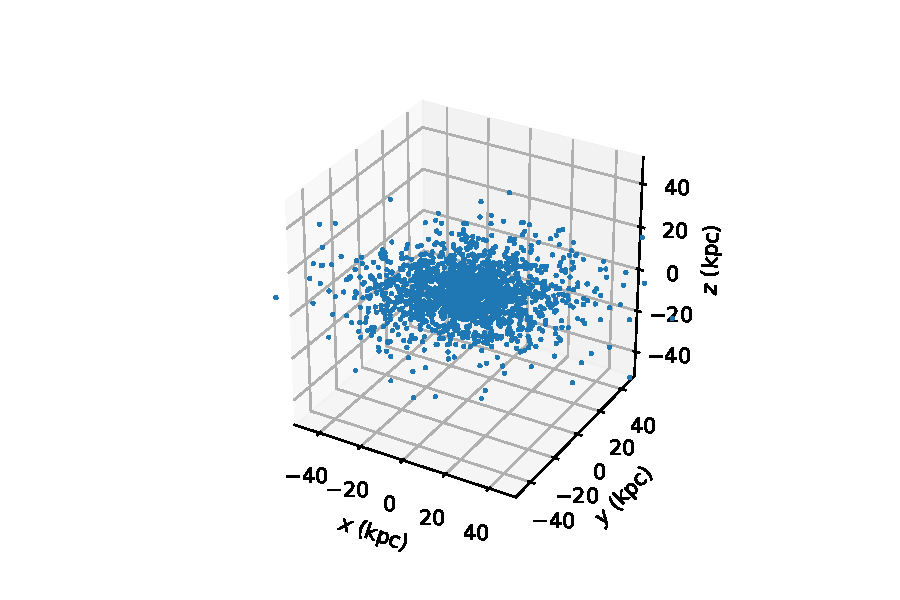
\includegraphics[height=0.35\textheight]{sources/images/galaxy_shape.pdf}\\\pause
			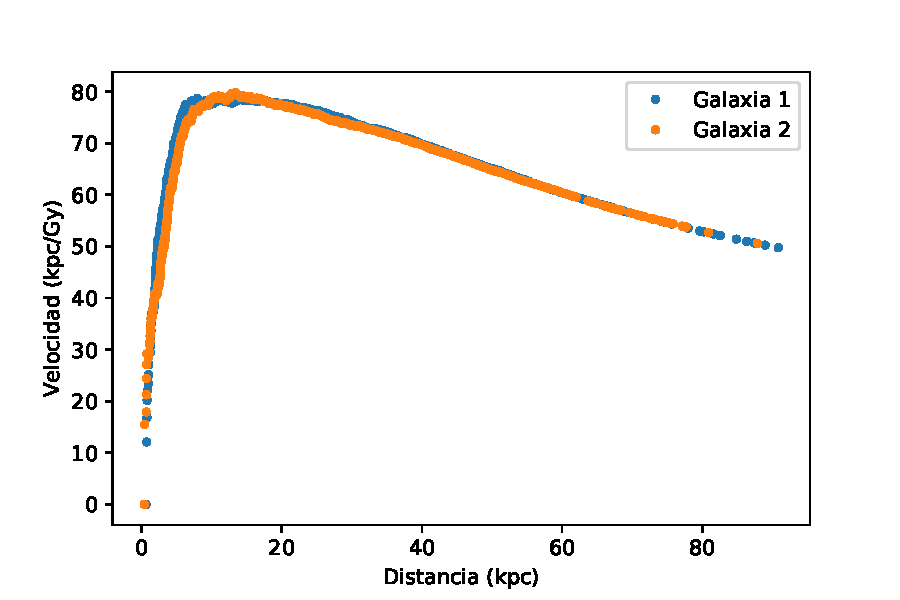
\includegraphics[height=0.35\textheight]{sources/images/rotation_curve.pdf}\pause
		\end{column}
		\begin{column}{0.65\textwidth}
			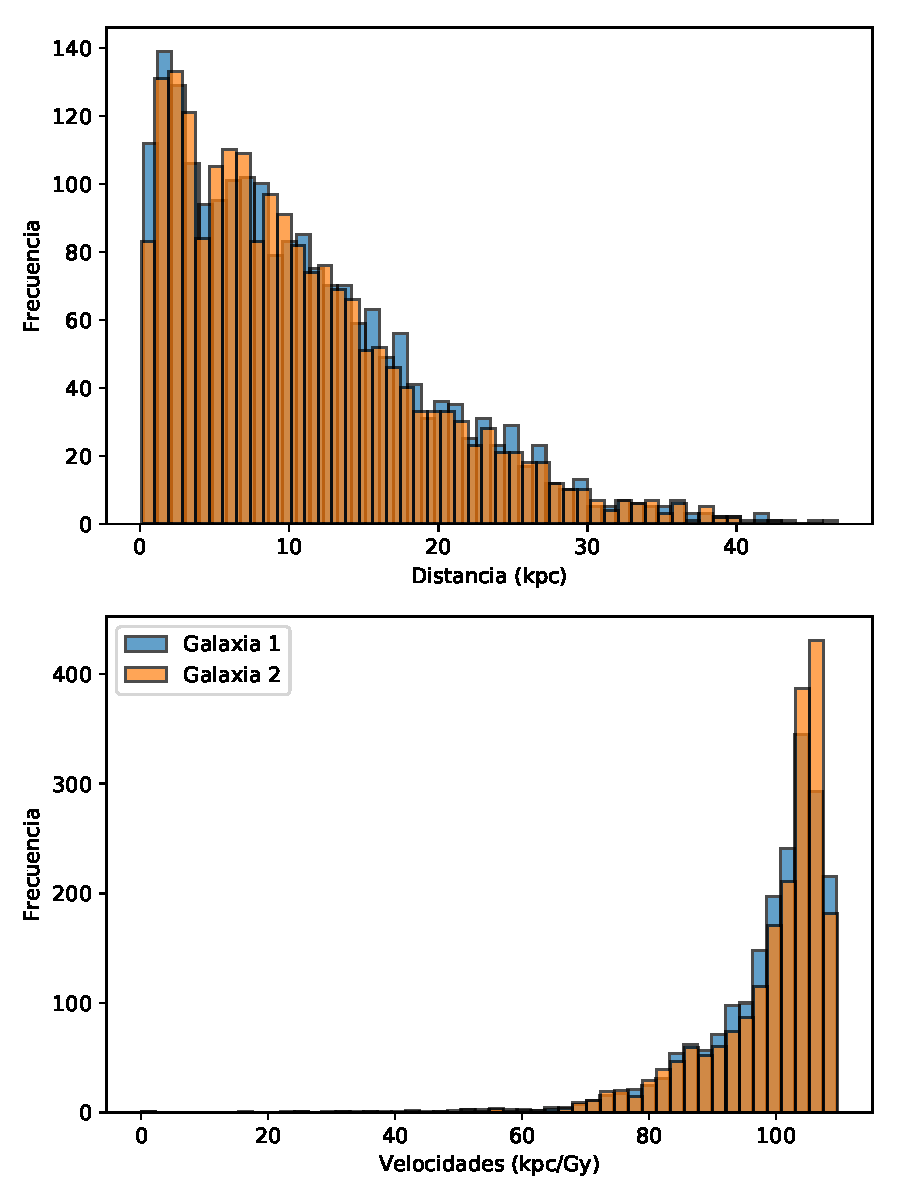
\includegraphics[width=\linewidth]{sources/images/galaxy_distribution.pdf}\\\pause
			\footnotesize
			\begin{itemize}
				\item $G$ = 44.97 (10$^7$ M$_{\odot}^{-1}$kpc$^3$Gy$^{-2}$)
				\item Tama\~no = 55 (kpc)
				\item $m$ = 2.44 (10$^7$M$_{\odot}$)
				\item $N$ = 4096
				\item $\epsilon$ = 0.055
			\end{itemize}
		\end{column}
	\end{columns}
\end{frame}
\begin{frame}{Soluci\'on de las ecuaciones}
	{\scshape Leapfrog}
	La soluci\'on num\'erica a las ecuaciones diferenciales se obtiene usando el m\'etodo de \textit{Leapfrog}, el cual avanza asincr\'onicamente en la posici\'on y la velocidad.
	\begin{equation}
		\begin{matrix}
			v_{i+1/2} = v_i + a_i\dfrac{\Delta t}{2}\\
			x_{i+1} = x_i + v_{i+1/2}\Delta t \\
			v_{i+1} = v_{i+1/2}+a_{i+1}\dfrac{\Delta t}{2}
		\end{matrix}
	\end{equation}
\end{frame}

\begin{frame}{Visualizaci\'on}
	La visualizaci\'on de los resultados puede ser \textit{cualitativa} o cuantitativa.
	\begin{columns}
		\begin{column}{0.5\textwidth}
			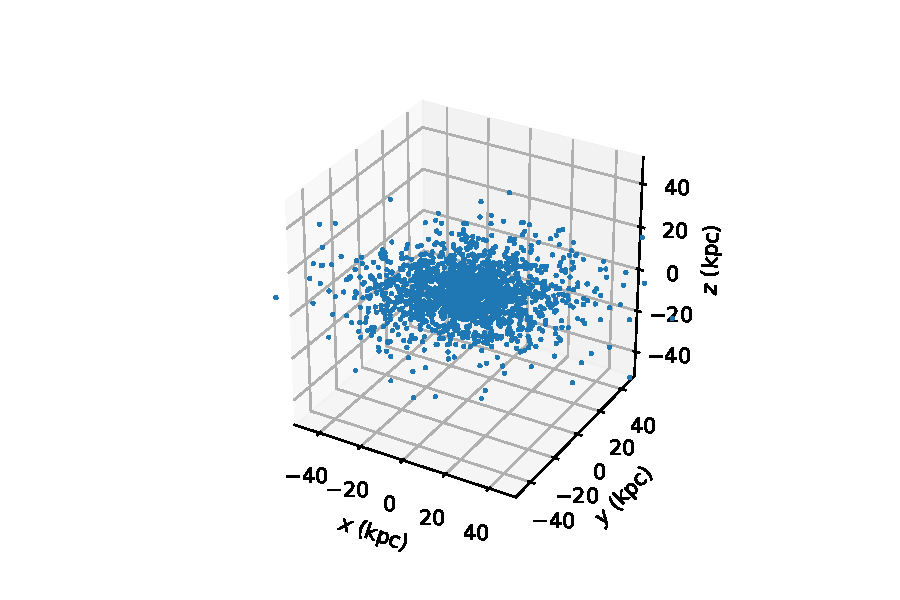
\includegraphics[height=0.35\textheight]{sources/images/galaxy_shape.pdf}
		\end{column}
		\begin{column}{0.5\textwidth}
			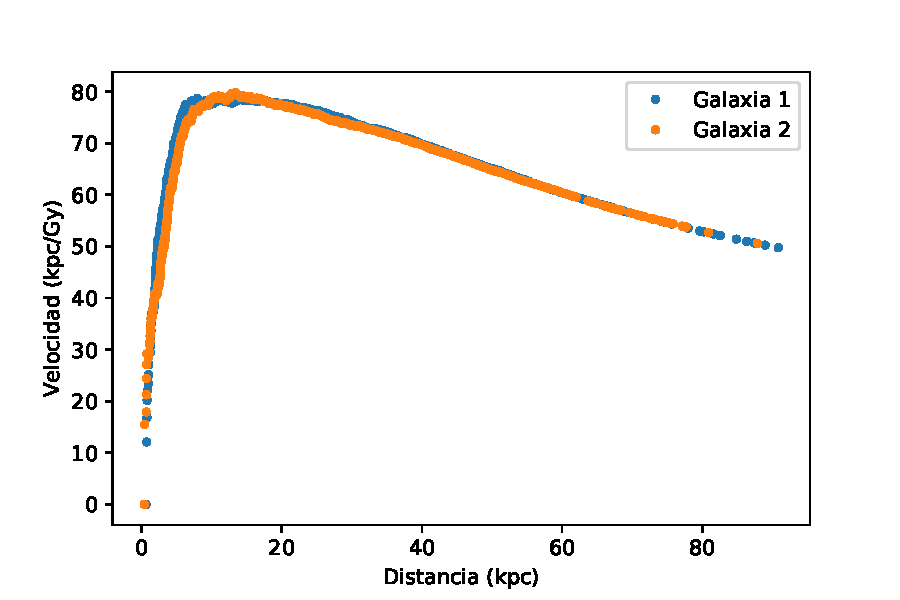
\includegraphics[height=0.35\textheight]{sources/images/rotation_curve.pdf}
		\end{column}
	\end{columns} 
\end{frame}
\begin{frame}{Implementaci\'on}
	Binding de \texttt{bruteforce.c} para Python.
	\begin{tcolorbox}[colback=green!5,colframe=green!40!black,title=C Programming Language]
		\begin{itemize}
			\item \texttt{init.c}: configura las variables globales de la simulaci\'on $(N, m, G, \epsilon, \tau)$, los arrays de posiciones y velocidades.
			\item \texttt{box.c}: contiene las funciones propias del \'arbol y sus cajas.
			\item \texttt{bruteforce.c}: resuelve las ecuaciones diferenciales, y genera archivos de datos.
		\end{itemize}
	\end{tcolorbox}
\end{frame}
\begin{frame}{Implementaci\'on}
	\begin{tcolorbox}[colback=blue!5,colframe=blue!40!black,title=Python]
		\begin{itemize}
			\item \texttt{core.py}: contiene la clase \texttt{Galaxy} y \texttt{Simulation}, las cuales generan condiciones iniciales y realizan la interf\'az con C.
		\end{itemize}
	\end{tcolorbox}
\end{frame}
\begin{frame}{Ejecuci\'on de la simulaci\'on}
	\begin{columns}
		\begin{column}{0.75\textwidth}
			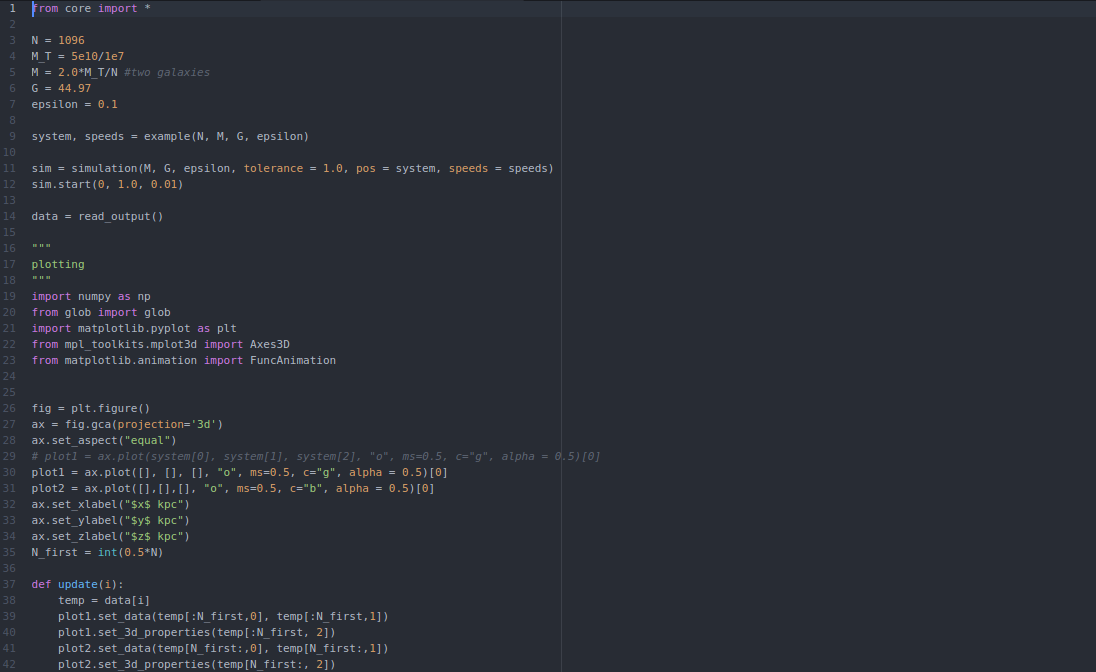
\includegraphics[height=0.5\textheight]{sources/images/code.png}
		\end{column}
		\begin{column}{0.25\textwidth}
			Python script
		\end{column}
	\end{columns}
	\begin{enumerate}
		\item \texttt{system, speeds = example(N, M, G)} \pause
		\item {\footnotesize\texttt{sim = simulation(M, G, epsilon, tolerance = 1.0, pos = system, speeds = speeds)}} \pause
		\item \texttt{sim.start(0.0, 1.0, 0.01)}
	\end{enumerate}
\end{frame}
\begin{frame}{Ejecuci\'on de la simulaci\'on}
	\begin{columns}
		\begin{column}{0.75\textwidth}
			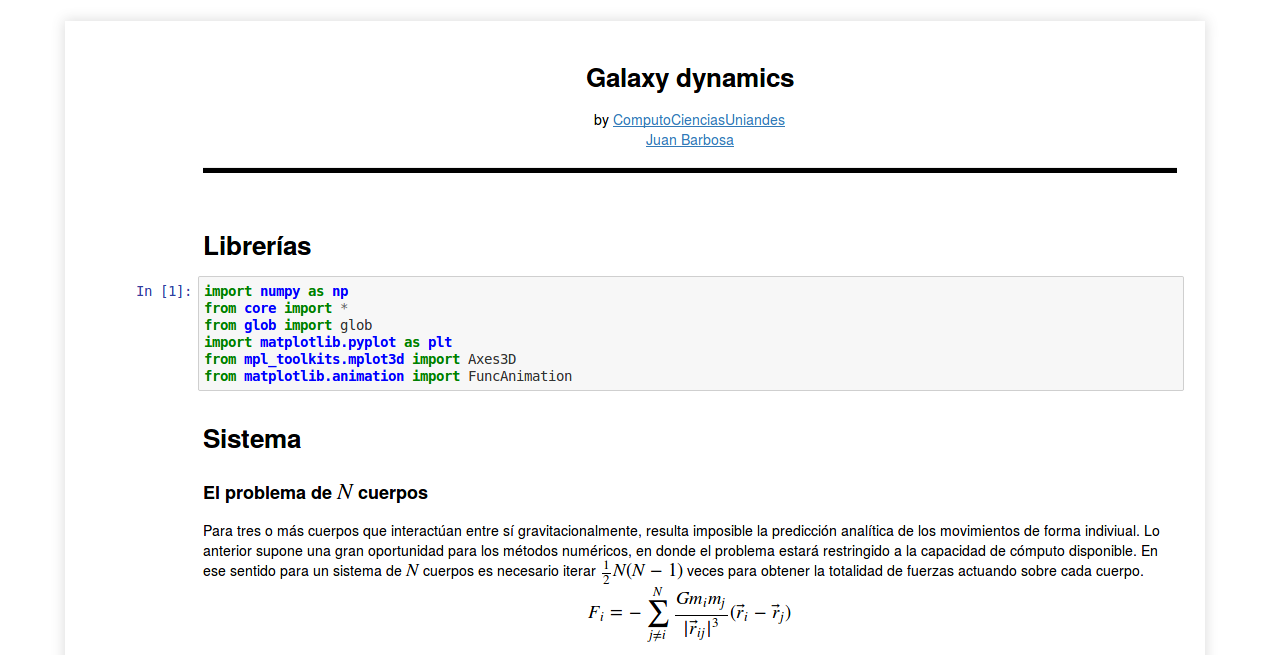
\includegraphics[height=0.5\textheight]{sources/images/screen.png}
		\end{column}
		\begin{column}{0.25\textwidth}
			Python Notebook
		\end{column}
	\end{columns}
	Disponible en:
	\tiny
	\url{https://github.com/ComputoCienciasUniandes/Demonstrations/tree/master/GalaxyDynamics}
	\normalsize
\end{frame}
\begin{frame}{Resultados}
	\centering
	\movie[height = 0.55\textwidth, width = 0.8\textwidth, poster, showcontrols]{}{sources/animations/exact.mp4}
	\\
\end{frame}
\begin{frame}{Resultados}
	\centering
	\movie[height = 0.55\textwidth, width = 0.8\textwidth, poster, showcontrols]{}{sources/animations/approx.mp4}
	\\
\end{frame}
\begin{frame}{Resultados}
	Efecto del coeficiente de precisi\'on en el tiempo de c\'omputo.
	\begin{columns}
		\begin{column}{0.5\textwidth}
			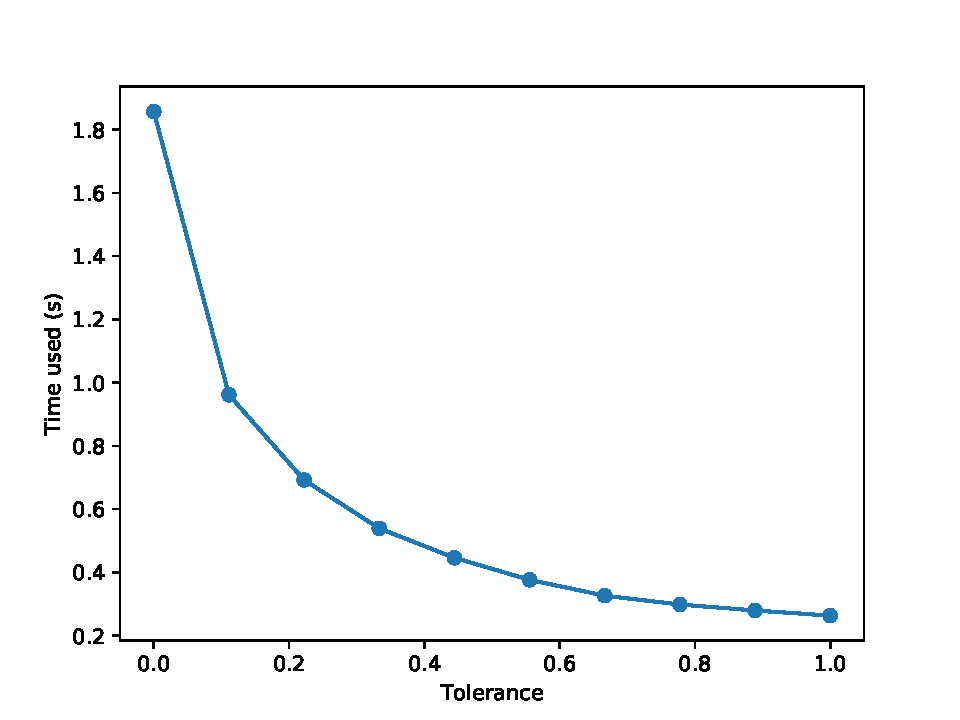
\includegraphics[width=\linewidth]{sources/images/Tolerance_results.pdf}
		\end{column}
		\begin{column}{0.5\textwidth}
			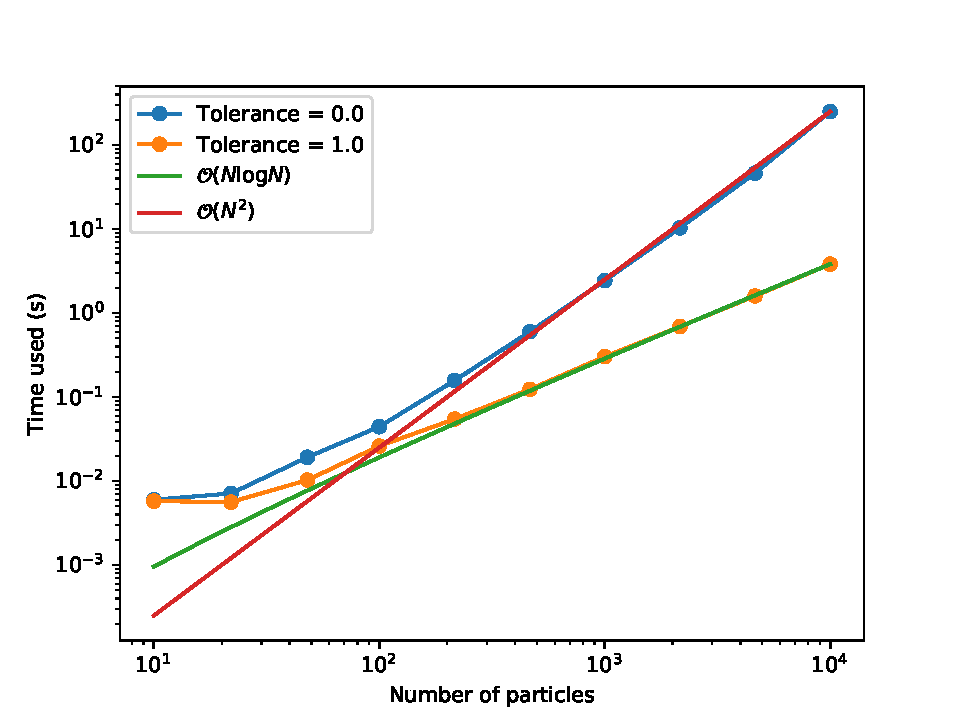
\includegraphics[width=\linewidth]{sources/images/Particles_results.pdf}
		\end{column}
	\end{columns}
\end{frame}
\begin{frame}{Conclusiones}
	Funciona.
\end{frame}
\end{document}